% Cue conflict in chain-of-thought arithmetic -- ARR short-paper draft (4 pages of body).
%
% NO EXPERIMENT HAS BEEN RUN. Every quantity is a \NUM{} placeholder that renders in red as
% <<name>>; scripts/51_tables.py writes numbers.tex as results land. The prose here is the part
% that does not depend on results: framing, setup, the outcome table, related work, limitations.
% Section 4 (Results) is written as the SHAPE of each paragraph with placeholders, per the
% outcome table in PLAN.md §5, so any of the four outcomes can be filled in without restructuring.
%
% Build: make paper   (tectonic at envs/tex/bin/tectonic; prints body page count vs limit 4)

\documentclass[11pt]{article}
\usepackage[review]{acl}      % anonymous + line numbers for ARR; final / preprint later
\usepackage{times}
\usepackage{latexsym}
\usepackage[T1]{fontenc}
\usepackage[utf8]{inputenc}
\usepackage{microtype}
\usepackage{inconsolata}
\usepackage{graphicx}
\usepackage{booktabs}
\usepackage{amsmath}
\usepackage{xcolor}
\usepackage{url}

% An unfilled number must be impossible to miss.  % grep-skip
\providecommand{\NUM}[1]{\textcolor{red}{$\langle\langle$\texttt{#1}$\rangle\rangle$}}
\providecommand{\tabinput}[1]{\IfFileExists{tables/#1.tex}{\input{tables/#1.tex}}{\textcolor{red}{[table \texttt{#1} not generated yet]}}}
\IfFileExists{numbers.tex}{% generated by scripts/51_tables.py -- do not edit
\expandafter\newcommand\csname NUMval@interferencellama323bcotv1\endcsname{2.0}
\expandafter\newcommand\csname NUMval@interferencellama323bcotv2\endcsname{-2.8}
\expandafter\newcommand\csname NUMval@interferencellama323bdirectv1\endcsname{-0.5}
\expandafter\newcommand\csname NUMval@interferencellama323bdirectv2\endcsname{-0.4}
\expandafter\newcommand\csname NUMval@lureratellama323bcotv1\endcsname{0.4}
\expandafter\newcommand\csname NUMval@lureratellama323bcotv2\endcsname{0.0}
\expandafter\newcommand\csname NUMval@lureratellama323bdirectv1\endcsname{8.6}
\expandafter\newcommand\csname NUMval@lureratellama323bdirectv2\endcsname{8.1}
\renewcommand{\NUM}[1]{\ifcsname NUMval@#1\endcsname\csname NUMval@#1\endcsname\else\textcolor{red}{$\langle\langle$\texttt{#1}$\rangle\rangle$}\fi}
}{}

\definecolor{neu}{RGB}{60,60,60}
\definecolor{con}{RGB}{0,110,60}
\definecolor{inc}{RGB}{180,30,30}

\title{Name or Value? Cue Conflict Reveals When Chain of Thought Overrides Lexical Priors}

\author{Anonymous ACL submission}

\begin{document}
\maketitle

\begin{abstract}
Language models are misled by variable names that contradict a program's behavior, but an
accuracy drop cannot show where inside the model the name interferes. Interpretability studies
find that intermediate values are computed during chain of thought, yet in their clean tasks the
variable name and the computed value never disagree. We introduce a cue-conflict test for
multi-step arithmetic in which each problem appears with congruent, neutral, and incongruent
variable names under identical arithmetic, and evaluate two Llama models across four difficulty
levels and three demonstration sets. Without a chain of thought the models read a variable's
value off its name: a congruent name raises accuracy by up to \NUM{facilitationmax} points and an
incongruent one yields the name's value as the answer up to \NUM{lureexcessmax} points above
chance. With a chain of thought the name's value has no measurable effect on the answer at any
level. Linear probes trained on neutral problems show that the lure is decodable only at the
name's own tokens and is erased at the step that writes the value; activation patching localises
the no-chain lure to the early-layer representation of the equation that defines the name.
Chain of thought thus overrides the lexical prior by replacing it, not by suppressing it. What a
chain does not remove is a word-class effect on equation selection, and every effect we measure
is smaller than the effect of which three demonstrations are shown.
\end{abstract}

\section{Introduction}

Models read code and mathematics in which names carry meaning, and names that contradict the
computation reduce accuracy: on real programs, removing or corrupting identifiers degrades
execution prediction \cite{le2025names}, misleading comments and hints cut output prediction by
a fifth \cite{lam2025codecrash}, and adversarial identifier renaming impairs comprehension through semantic displacement and interference in a prior human--model study \cite{le2026obfuscated}. An accuracy drop, however, is compatible with three
different failures: a corrupted input representation, a corrupted computation, or a correct
computation misread at output, and these differ in whether a written chain of thought can be
trusted and in how the failure might be fixed.

Interpretability work on clean tasks cannot separate them either. \citet{kudo2026faithful} show,
with linear probes and activation patching on controlled multi-step arithmetic, that the values
of intermediate variables become linearly decodable only as the chain of thought is written, and
that the final answer depends causally on the chain. But in their tasks the variable names are
letters. The decoded value has exactly one possible source, so nothing in the design can tell
``the model computed 5'' from ``the model read 5 off a cue,'' because no cue ever disagrees.

Cue conflict resolves this. In the Stroop task \cite{stroop1935}, the word \textsc{red} printed
in blue ink reveals whether reading overrides colour naming; in vision, shape--texture conflict
images showed that apparent shape recognition in CNNs was partly texture matching
\cite{geirhos2019texture}. We bring the design to arithmetic reasoning. Every problem appears
in three matched versions with identical arithmetic (Figure~\ref{fig:one}):
\textcolor{neu}{neutral} names (\texttt{pen=1 + cup, cup=2 + 3; pen=?}),
\textcolor{con}{congruent} names, where a number word equals the variable's true value
(\texttt{five=2 + 3}), and \textcolor{inc}{incongruent} names, where it does not
(\texttt{two=2 + 3}, true value 5, lure 2). Each version is solved with and without a written
chain of thought, and linear probes trained on neutral problems only read out, at every layer
and reasoning step, whether the representation holds the true value or the lure.

Our main finding is that the chain overrides the name by replacement: without a chain of
thought the models use the name's value as a shortcut in both directions, with a chain the value
of the name is irrelevant to the answer, and inside the model the lure is present only where the
name sits and disappears at the step that computes the value. Concretely, we contribute (i) a
cue-conflict extension of a controlled arithmetic benchmark with matched twins, generation rules
that make the lure never correct for another reason, and the demonstration set as a reported
factor; (ii) a layer, position and reasoning-step map of lure versus true value, with and without
chain of thought, on two models and four levels; and (iii) causal evidence from activation
patching with two control patches on where the no-chain lure lives.

\begin{figure}[t]
\centering
\fbox{\parbox{0.95\columnwidth}{\small
\textcolor{neu}{\texttt{pen=1 + cup, cup=2 + 3; pen=?}}\\
\textcolor{con}{\texttt{pen=1 + five, five=2 + 3; pen=?}}\\
\textcolor{inc}{\texttt{pen=1 + two, two=2 + 3; pen=?}}\\[2pt]
\texttt{\ \ \ \ pen=1 + two, two=2 + 3, two=5, pen=1 + two, pen=1 + 5, pen=6}\\[2pt]
\textit{[margin sketch: $\log p(\text{true})-\log p(\text{lure})$ across P2--P5, to be drawn
from a real instance once probes exist]}}}
\caption{One problem in its three matched versions (top), the chain of thought with probe
positions P2--P5 (middle), and the probe margin across reasoning steps (bottom). The
incongruent name \texttt{two} has true value 5 and lure value 2.}
\label{fig:one}
\end{figure}

\section{Setup}

\paragraph{Task.} We reuse the generator, difficulty levels and prompt format of
\citet{kudo2026faithful}: problems are lists of assignments over single digits with $+$ and $-$,
all values stay in $0..9$, and three fixed same-level demonstrations precede each problem. Our
main level is their Level~3 (two steps, one forward reference; \texttt{v1=d $\pm$ v2, v2=d $\pm$ d; v1=?}),
with Levels 2 and 5 as robustness checks and Level~4 for a control described below. Probes are
trained on 10,000 neutral problems; evaluation uses 2,000 matched sets per level with the
probe-training digit expressions held out.

\paragraph{Conditions.} Each arithmetic problem yields a matched set. The \emph{letter}
condition is Kudo et al.'s format and anchors our replication. \emph{Neutral} names are common
single-token words. In the \emph{congruent} and \emph{incongruent} conditions exactly one
variable, the target, is renamed to a number word that equals or does not equal its true value.
The target is either the intermediate variable or the queried one. An \emph{irrelevant-lure}
control at Level~4 gives the number-word name to a distractor outside the queried chain,
separating the lexical presence of a number from a binding conflict.

\paragraph{Generation rules.} Exactly one variable per instance carries a number word. The
lure differs from every variable value and from every operand digit in the problem, so it is
never correct for another reason. Neutral words are common concrete nouns that are a single token in
every context of the template under each model's tokenizer (Appendix~A), so twins tokenize to
identical layouts and length is not a confound. Every incongruent instance has a neutral and a congruent twin with identical
arithmetic, and all comparisons are within these sets.

\paragraph{Regimes.} In the \emph{chain-of-thought} regime the model writes each step in Kudo
et al.'s format (\texttt{cup=5, pen=1 + 5, pen=6}); note that the chain writes the name next to
the computed value, which may help the model recover. In the \emph{direct} regime it writes only
\texttt{pen=6}. The contrast between regimes is the center of the paper.

\paragraph{Probe positions.} P1, the name token \texttt{two} at its definition, decodes the
lure trivially and is a reference only. P2 is the last operand of the definition, the first
position where the true value can be computed; P3 the query position before any chain; P4 the
chain position where the target's value is about to be written; P5 the final answer position.
All claims about lure interference are made at P2--P5.

\paragraph{Probes and patching.} Probes are single linear layers trained with
\citeauthor{kudo2026faithful}'s recipe on the neutral condition only, then evaluated on
congruent and incongruent instances; training on incongruent data would let the probe learn the
lure. We report accuracy for the true value, the \emph{lure mass} (probability on the lure
class), and the \emph{margin} $\log p(\text{true})-\log p(\text{lure})$; the \emph{crossover}
is the first step at which the margin becomes and stays positive. Selectivity against a control
task \cite{hewitt2019control} accompanies every probe, over three seeds. For causation we patch
residual-stream activations at the misleading name's token positions from the matched neutral
twin into the incongruent run \cite{zhang2024patching}, sweep layers, and measure the
\emph{recovery rate}, the share of lure errors that become correct. A patch from a different neutral word
measures patching damage; a patch from a different lure tests whether the answer follows it.

\paragraph{Models.} \NUM{model-list}, base models of 3B and 8B parameters from
\citeauthor{kudo2026faithful}'s panel, plus \NUM{extra-models}. Behavioural metrics are
accuracy, lure rate (answers equal to the lure), \emph{interference} (neutral minus incongruent
accuracy) and \emph{facilitation} (congruent minus neutral), with cluster-bootstrap confidence
intervals over matched sets.

\section{Results}

\paragraph{Replication.} On the letter condition our per-token probes reproduce
\citeauthor{kudo2026faithful}'s Table~3 for Llama-3.2-3B exactly: the queried variable becomes
decodable at equation 5 of the chain and the intermediate at equation 2, with pre-chain maxima
of \NUM{replication-pre-v1} and \NUM{replication-pre-v2} (theirs: 17.8 and 33.2).

\paragraph{RQ1: behaviour.} Table~\ref{tab:behavior} reports, per model and regime, accuracy
and the pre-registered contrasts pooled over three demonstration sets, with a contrast claimed
only when its sign holds in every set. Without a chain the name's value is used as a shortcut:
a congruent name on the queried variable adds \NUM{facilitationllama318bdirectv1} points for
Llama-3.1-8B at level 3 and up to \NUM{facilitationmax} points at level 5, and an incongruent
name yields lure answers \NUM{lureexcessllama318bdirectv1} points above chance at level 3 and up
to \NUM{lureexcessmax} points where accuracy is at floor. With a chain the same contrasts are
within \NUM{chain-lure-bound} points of zero in every cell, and congruent and incongruent names
move together. The irrelevant-lure control at level 4 separates presence from binding: a number
word on the distractor costs accuracy but produces no lure answers. What the chain does not
remove is a word-class effect: a number-word name on the queried variable at level 4 costs
Llama-3.2-3B \NUM{interferencellama323bcotv1} points whether or not its value agrees, and the
error analysis shows the model restating the wrong equation next.

\begin{table}[t]
\centering\small
\resizebox{\columnwidth}{!}{\tabinput{behavior}}
\caption{Accuracy (\%), lure rate, interference and facilitation per model, regime and target
position, Level~3, pooled over three demonstration sets with 95\% cluster-bootstrap intervals
over matched sets.}
\label{tab:behavior}
\end{table}

\paragraph{RQ2: representation.} Figure~\ref{fig:heat} maps the probe margin over layers and
positions P2--P5 in the incongruent condition, chain of thought beside direct answer. At P2, the
end of the defining equation, the true value is already partly computed (accuracy
\NUM{p2-acc}, selectivity \NUM{p2-sel}) and the lure is weak (lure rate \NUM{p2-lure}). At P3,
the query, a neutral-trained probe reads the lure in \NUM{p3-lure} of instances, but the control
task scores \NUM{p3-ctl} there: the readout is the name's identity, not a value, and we do not
claim it. At P4 and P5 the true value is decodable at \NUM{p4-acc} with the lure at zero in
every condition and level; per-token probes show the lure decodable only at the name's own
tokens, and a number word bound to a computed variable has lure mass \NUM{bound-mass} at the
answer against \NUM{unbound-mass} for an unbound one on the distractor. The outcome cell is
``lure fades, answer correct'', reached by replacement at the value step rather than suppression.

\begin{figure}[t]
\centering
\IfFileExists{figures/fig2_margin_llama32-3b_L3_v2.pdf}{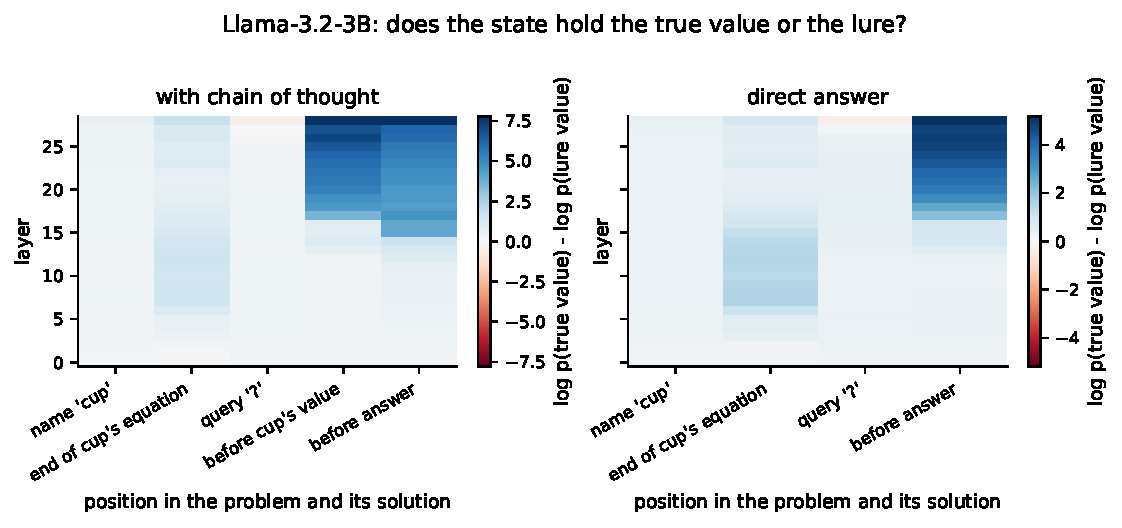
\includegraphics[width=\columnwidth]{figures/fig2_margin_llama32-3b_L3_v2.pdf}}{\fbox{\parbox{0.95\columnwidth}{\centering\small\textcolor{red}{[Figure 2: margin heatmap, generated by scripts/52\_figs.py]}}}}
\caption{Probe margin $\log p(\text{true})-\log p(\text{lure})$ by layer and position, incongruent
condition, chain of thought (left) and direct answer (right), Llama-3.2-3B. Positive means the
true value dominates.}
\label{fig:heat}
\end{figure}

\paragraph{RQ3: causation.} Figure~\ref{fig:patch} plots, for the direct regime, the share of
lure errors removed by patching the name's tokens from the matched neutral twin, by layer, with
the two controls. For Llama-3.2-3B the neutral patch removes \NUM{lure-removed-3b} of lure
errors and restores the true-minus-lure margin fully (normalised logit difference
\NUM{nld-3b}), the alternative-lure patch is followed in \NUM{follow-new-lure} of cases, and the
span grid places the effect in the defining equation at layers \NUM{grid-layers}. The word
control changes \NUM{control-damage} of correct answers at this floor accuracy, so we report the
localisation and not a recovery rate. For Llama-3.1-8B the no-chain lure rate at level 3 is at
chance and both patches behave alike; the effect exists only where the lure does. With a chain
there are no lure errors to patch and both controls are clean.

\begin{figure}[t]
\centering
\IfFileExists{figures/fig3_patching_llama32-3b_L3_v2.pdf}{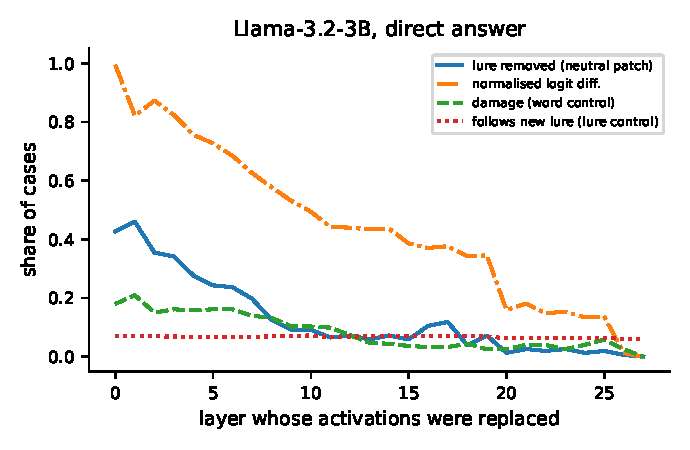
\includegraphics[width=0.8\columnwidth]{figures/fig3_patching_llama32-3b_L3_v2.pdf}}{\fbox{\parbox{0.95\columnwidth}{\centering\small\textcolor{red}{[Figure 3: patching by layer with controls, generated by scripts/52\_figs.py]}}}}
\caption{Lure errors removed by patching the name's tokens from the neutral twin, by layer,
direct regime, with the neutral-word control patch (damage) and the alternative-lure patch.}
\label{fig:patch}
\end{figure}

\section{Related Work}

\citet{kudo2026faithful} established when sub-answers are computed during chain of thought on
clean arithmetic; we add cue conflict to ask what that computation is sensitive to. Two recent
studies bring the Stroop design to language models: \citet{wang2026stroop} pits a local
redefinition of a word against its familiar associate and restores the lost margin by patching
from a matched neutral prompt; \citet{hu2026conflict} read a congruency effect off next-token
probabilities in a colour-rule task every model solves. Both measure one next token; neither has
errors, a chain of thought, or probes over reasoning steps. Faithfulness has been measured from
the outside by perturbing prompts, chains or parameters
\cite{turpin2023unfaithful,lanham2023measuring,chen2025reasoning,tutek2025unlearning}; we
measure it inside the model under a cue whose true and lure values are both known. On
arithmetic, \citet{liu2026readout} show that small models copy the trailing chain number and
\citet{prabhakar2024deciphering} that an output prior can override a correct chain; our
late-readout outcome is stated against a positional-copy control. Misleading identifiers and
comments hurt on real code \cite{le2026obfuscated,le2025names,lam2025codecrash}; we trade
realism for localisation. Binding work asks how a value attaches to a name
\cite{feng2024binding,wu2025binding,gurarieh2026mixing}; we ask whether the attachment survives
a name carrying a competing value. \citet{shi2023distracted} add irrelevant context; here the
distractor is the name itself. The design is \citet{stroop1935} and \citet{geirhos2019texture}.

\section{Conclusion}

A misleading variable name is used when the model has nothing better: without a chain of
thought the name's value becomes the answer, with a chain it is replaced at the step that
computes the value and never reaches the output. For faithfulness this is the reassuring cell of
the outcome table, and it comes with two cautions: the chain leaves a word-class effect on which
equation the model attends to next, and the demonstration set moves accuracy more than any name.

\section*{Limitations}

The task is synthetic arithmetic with short chains, so the results need not transfer directly to
real code, which is the motivation and not the finding. Models are at most 8B parameters;
within-family comparisons give the direction of the trend only. Lures are hand-picked English
number words; digit-bearing names such as \texttt{x2}, other languages and optimised lures are
future work. Linear probes can miss nonlinearly encoded information; the patching experiment
partly addresses this, but hidden states carry mixed information and patching cannot rule out
side effects entirely, which is why two control patches are reported. The chain-of-thought
format writes the name beside the computed value at every step, which may itself aid recovery;
the direct regime bounds that effect from the other side.

\bibliography{refs}

\appendix
\section{Tokenizer checks}
Per-model lists of neutral words that are one token in every context (line start, after a
comma, as an operand), and the token layout of the template: \NUM{appendix-tokenizer}.
\section{Full layer sweeps and selectivity}
\NUM{appendix-sweeps}
\section{Additional models and levels}
\NUM{appendix-models}

\end{document}
